\chapter{Introduction}
Understanding the evolution and structure of stars is one of the main challenges in modern astrophysics. Fundamental properties of stars such as radius, mass and temperature need to be measured in order to compare them to predictions made using stellar models. 
Advances in understanding stars are driven by ever more precise measurements which can test the theories behind the models. Interferometry and asteroseismology are amongst the most powerful tools we have for this. Interferometry allows an almost-direct measurement of the physical size of star, although it can only be applied to the brightest stars. Asteroseismology enables us to infer stellar properties by measuring the variety of waves travelling through the stellar interior. 
Ideally both methods can be used in order to find the constraints needed for stellar modelling and thus to test -- and improve -- our current models of stellar structure and evolution.

The aim of this project is to determine the radius of a subgiant star from interferometry and then compare with a radius determined from asteroseismology. 
The subgiant star of interest is \mystar. This star has not been the subject of detailed studies before, but has mostly been used as a comparison star in spectroscopy and photometry \citep{schiller1988photometric,ferrero2004magnetic}.
The entire process from raw data to radius of the star using both asteroseismology and interferometry will be explained and discussed in this project.

In this chapter, the theoretical background for interferometry and asteroseismology is introduced. 
Sec.~\ref{sec:principleinterferometry} present the basics of interferometry.

\vspace{-5pt}
\section{The Principle of Interferometry}
\label{sec:principleinterferometry}
\vspace{-5pt}
Interferometry is an observational method in which the interference of electromagnetic waves is used to obtain the greatest possible angular resolution. 
%The underlying principle is the wave nature of light and the interference of these waves. 
A full and detailed review is given by  \citet{lawson2000principles} and \citet{monnier2003optical} upon which this section is based.
\plainbreak1
The fundamental principle of the interference of light can be nicely illustrated by Young's double slit experiment. In this experiment, monochromatic light from a distant point source illuminates a plate with two parallel, narrow slits separated by a distance~$B$.
The light travels through this double-slit assembly and towards the detection screen on the other side. According to Huygens's principle, every point of the wave front may be considered as a source of secondary spherical wavelets with a speed equal to the propagation speed of the wave. These wavelets interfere with one another, creating an interference pattern on the detection screen.
\begin{figure}
	\centering
	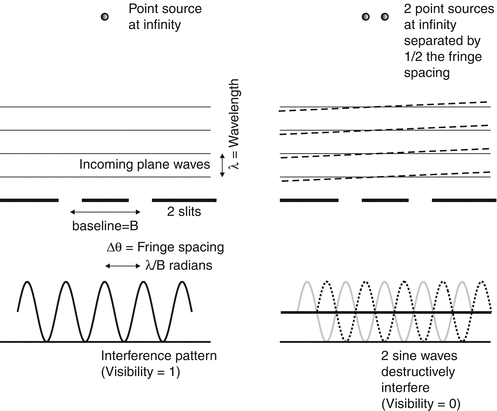
\includegraphics[width=1\linewidth]{./figures/fig72monnier2003-cropped}
	\caption{Two scenarios: the case of a single point-like light source, and the case of two point sources, separated by an angle of half the fringe spacing. The visibility is one and zero respectively due to interference. Figure from \citet{monnier2003optical}.}
	\label{fig:fig72monnier2003}
\end{figure}
Because the wavelets all have the same frequency, the resulting pattern is determined only by the phase difference between two waves. If the two waves are in phase (anti-phase) when they hit the detection screen, they will interfere constructively (destructively) and produce a bright (dark) patch. 
%If the two waves are in anti-phase, destructive interference will occur and appear as a dark patch. 
From the grating equation, the angular spacing between the bright and dark spots $\Delta \Theta$ can be approximated as
\begin{equation}
\label{eq:angularspacing}
\Delta \Theta \approx \frac{\lambda}{B},
\end{equation}
where $\lambda$ is the wavelength of the light and $B$, as mentioned earlier, denotes the distance between the slits. This distance is also called the baseline, hence the symbol $B$. 
%Imagine the scenario in which a second point-like light source of equal brightness as the first also illuminates the plate and this second light source is placed at exactly half a fringe spacing,  ${\Delta \Theta}/{2} = {\lambda}/{2 B}$, in angular distance from the first light source as seen from the plate as shown in \figref{fig:fig72monnier2003}. 
%In two-telescope interferometry, the two slits in Young's experiment are replaced by two telescopes, and we could imagine two point-like sources as two stars far away. 
In \figref{fig:fig72monnier2003}, a second point source of equal brightness as the first is placed at half a fringe spacing,  ${\Delta \Theta}/{2} = {\lambda}/{2 B}$, in angular distance from the first light source as seen from the plate. 
The combined light from these point sources will interfere destructively at all points  on the screen since the fringes are in exact anti-phase, and therefore, no contrast between bright and dark spots is visible.
%Therefore the combined light will show no contrast between bright and dark spots; the detection screen will just be evenly illuminated. 

This suggests that the contrast between the dark and bright patches in the interference pattern at a given wavelength and baseline is directly related to the structure of the observed object. 
The pattern is affected by the angular separation of two point sources or the angular extent of a single extended object. More precisely, the fringe contrast or the visibility $V$ can be defined as the ratio between the fringe amplitude (i.e.\@ half the difference between the maximum and minimum intensity $ (I_{\text{max}}-I_{\text{min}})/2$) and the average intensity:
\begin{equation}
V = \frac{I_{\text{max}}-I_{\text{min}}}{I_{\text{max}}+I_{\text{min}}} = \frac{\text{Amplitude}}{\text{Average intensity}}. 
\end{equation}
In the case of total constructive (destructive) interference, the visibility is one (zero).
%The Van Cittert-Zernike theorem relates more generally the complex fringe visibility $Q$ to a unique spatial Fourier transform of the intensity distribution of an object, see \citet{bradt2004astronomy}.
% $I(\vecb{\alpha})$:
%\begin{equation}
%Q(\vecb{\beta}) = \frac{\int I(\vecb{\alpha}) e^{-2\pi\vecb{\alpha}\vecb{\beta}}\dx{\vecb{\alpha}}}{\int I(\vecb{\alpha})\dx{\vecb{\alpha}}},
%\end{equation}
%where $\vecb{\alpha}$ is a given set of two-dimensional image coordinates and $\vecb{\beta}$ is the so-called spatial frequency, defined as the projected baseline vector $B$ (projection of the vector from telescope a to telescope b) scaled by the wavelength of the observation $\lambda$. A detailed review can be found in \citet{bradt2004astronomy}.
If the fringe visibility of an object is measured at different spatial frequencies, the spatial structure of the light source may be exposed \citep{van1934wahrscheinliche,zernike1938concept}. The spatial frequency $\beta$ is defined as the projected baseline $B$ in units of the wavelength $\lambda$
\begin{equation}
\label{eq:spatialfreq}
\beta = \frac{B}{\lambda}.
\end{equation} 
If the object in question is a star, measuring $V$ as a function of $\beta$ makes it possible to measure the angular diameter of the star. 
